\section{Tips for Emails and Reports}

% https://graphthinking.blogspot.com/2020/09/identifying-and-eliminating.html


%***************************

\subsection*{Why written communication does not happen\label{sec:written-comm-does-not-happen}}
\begin{itemize}
    \item Too many reports, emails, and messages to read and process and respond to. Bureaucrats feel emotionally and cognitively overwhelmed.
\item The receiving bureaucrat may read slowly.
\item The bureaucrat-as-author may type slowly, or their hand writing is poor.
\item Potential participants fear imperfect communication. What if the email is incomplete or inaccurate or ambiguous?
\item The bureaucrat views written communication as ``official" or ``plan of record'' and does not feel comfortable brainstorming or creating contingency plans.
\item The bureaucrat wants to avoid accountability for their statements.
\item The bureaucrat may not be confident in their writing ability -- spelling, grammar, sentence composition, structuring content. \footnote{For tips on writing, see 
\href{https://en.wikipedia.org/wiki/The_Elements_of_Style}{The Elements of Style}
\index{Wikipedia!\href{https://en.wikipedia.org/wiki/The_Elements_of_Style}{The Elements of Style}}, 
\href{https://www.youtube.com/watch?v=vtIzMaLkCaM}{LEADERSHIP LAB: The Craft of Writing Effectively} and \href{https://www.youtube.com/watch?v=aFwVf5a3pZM}{LEADERSHIP LAB: Writing Beyond the Academy},
and
\href{https://www.google.com/search?q=dodm+5110.04}{DoDM 5110.04, Manual for Written Material}}
\end{itemize}


%***************************

\subsection*{Email and Reports do not Constitute Communication}
Asynchronous communication has no requirement of a response or action. That's what makes it asynchronous. Any communication that occurs is merely incidental.

\ \\
\textit{Written documents as notifications}: Email can be used to document that you told someone something. 

\ \\
\textit{Email as a task request}: Putting a task in another person's queue may or may not be read, and may or may not be acted upon. 




%***************************

\subsection*{Email: A Piece of Art, A Form, and A Game\label{sec:art-form-game}}


\textbf{Email is Structured}: Originality is not a requirement in bureaucratic writing. Plagiarism is acceptable. The consistency of a 
\href{https://en.wikipedia.org/wiki/Mad_Libs}{Mad Libs} 
\index{Wikipedia!\href{https://en.wikipedia.org/wiki/Mad_Libs}{Mad Libs}}
template is efficient.  

\ \\
\textbf{Email is a Piece of Art}: Effort invested in each email to improve readability means more than careful wording. 
Use visual cues (different fonts, different font sizes, highlighting, font color) and pictures to improve readability. See figure~\ref{fig:email_computer_font} for example.

\ \\
\textbf{Email is a Game}: Email is a game of documenting decisions and responses so that the sequence of interactions is clear for audits and recrimination. 

\subsection*{Asynchronous Communication Responsiveness\label{sec:email-responsiveness}}

Delayed response applies to any asynchronous communication such as voicemail, email, memos, reports. Here I'll use email, though the same issues apply to other channels.


There are tiers of responsiveness, assuming the reader wants to respond but doesn't have sufficient time available.
(The explanations below can be the other side of \gls{stonewalling} or \gls{slow rolling}.)

Which level you are at depends on the speed of your reading, how fast you can write, number of incoming emails, number of outgoing emails, and how much time you allocate for email. 
\begin{enumerate}
    \item You are able to read all incoming emails and reply to all emails that necessitate a response.
    \item You are able to read all emails and reply to some. 
    \begin{itemize}
        \item Only the subset that are important.
        \item Only the subset that have short answers.
    \end{itemize}
    \item You are unable to read all incoming emails. 
    \begin{itemize}
        \item Skim content of all to find relevant information, but likely to miss some key points.
        \item Read email from important people only (based on sender).
        \item Search through inbox if someone needs something and cites an email that was sent.
    \end{itemize}
    \item You have an assistant to respond to emails.
    \item You have a front office team to handle messaging.
\end{enumerate}
The following scenarios are focused on case 2, where you are able to triage (skim) emails but do not have enough time to respond to each.


In a situation where you have insufficient time, which of the following emails do you reply to? An email from your boss, an email from your peer, an email from a person who reports to you, or a person who you do not know?
(The ratio of these email categories is not one to one to one to one.)

The email from your boss is likely the top priority. Of the remaining emails (peer, subordinate, unknown), the peer email is likely the next priority.
The subordinate and unknown person are likely last.

The consequence of triage is that when there's insufficient time available, your transparency to subordinates and unknown people is likely to decrease. 

\ \\
Let's consider another scenario requiring triage of email. Three emails come in. One has no action, one is easy to reply to, and the third is difficult and takes time. Which one gets the response?
As with the previous scenario, the ratio of these inbound emails is not one to one to one.

The email that is easy to reply to gets answered first.  The email that is difficult is second.
If you only have time for one of the emails, it's likely to be the easy one. This is an example of 
\href{https://en.wikipedia.org/wiki/Ambiguity_aversion}{ambiguity aversion}.
\index{Wikipedia!\href{https://en.wikipedia.org/wiki/Ambiguity_aversion}{ambiguity aversion}}
As a consequence, outsiders see this as you demonstrating bike-shedding; also known as the
\href{https://en.wikipedia.org/wiki/Law_of_triviality}{law of triviality}.
\index{Wikipedia!\href{https://en.wikipedia.org/wiki/Law_of_triviality}{law of triviality}}



\subsection*{Email Tips\label{sec:email-structure}}

\index{list of tips!Email}

Whether you are the only recipient or one of many receivers can change the intent of the email. Whether you are in the ``to" or ``cc" field matters. Unfortunately, ``to" versus ``cc" are not reliable indicators since email senders do not reliably conform to the expected use. 


%This categorization of text within emails is a useful natural language processing challenge for machine learning. Currently a few email providers already do some of this with identifying meeting logistics, providing reminders to follow-up, and providing reply snippets. A browser plug-in that differentiates the various purposes of text could help readers determine relevant actions and responses. 

An email sent to multiple recipients may have different purposes for different readers. The reader's role or knowledge may factor into how they interpret the content. The inclusion or exclusion of recipients alters how the content is understood. 

\textit{Email Tip}: Good emails balance enough context (the why) and relevant details (the what) against conciseness (word count). 

\ \\
\textit{Email Tip}: Emails convey both emotional tone and facts. Your intent as an author is practically irrelevant; the reader's perception is paramount. 


% from https://graphthinking.blogspot.com/2021/10/structuring-email-content-for.html

\ \\
\textit{Email Tip}: Use consistent design and structure for your emails. Emails are part of your professional reputation.

\ \\
\textit{Email Tip}: Emails start with a greeting: Hi, Hello, Good morning, Good afternoon, Good evening. 
Email greetings include the name of the targeted recipient(s). 

\ \\
\textit{Email Tip}: Emails end with a professional closing, e.g., ``Kindly", ``Regards", etc.

\ \\
\textit{Email Tip}: Emails have a signature block with contact information -- phone number, normal hours of response, which timezone you're in if your team spans timezones, how long to wait for a response before asking again, which communication channel I prefer, etc.

\begin{figure}
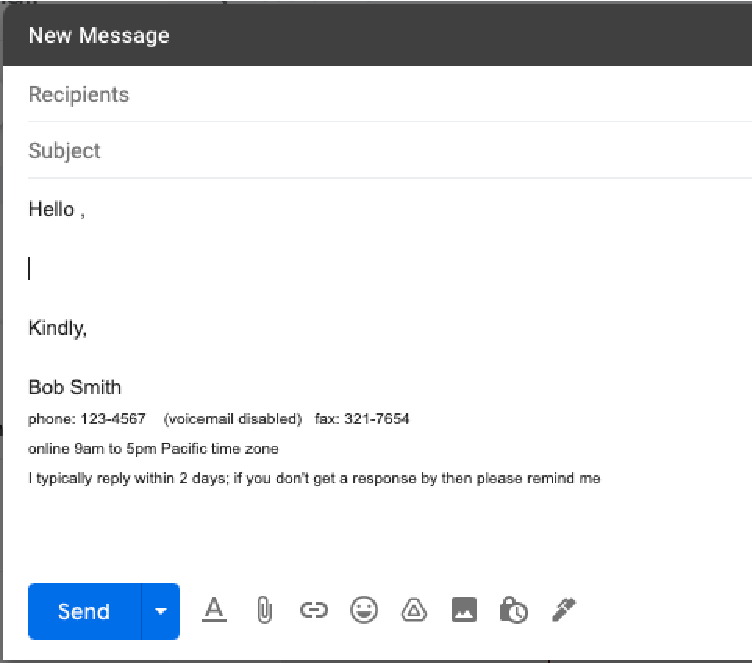
\includegraphics[width=1\textwidth]{images/email_template.pdf}
\caption{Template for new email messages. Greeting has a space after the comma -- that is where the recipient's name will go. Signature block uses smaller after the name.}
\label{fig:email_template}
\end{figure}

\ \\
\textit{Email Tip}: Email signature blocks do not include unnecessary images, as that uses more storage for recipients. 
Email threads focused on a specific instance of a recurring event include the date (YYYY-MM-DD) in the subject line. 

\ \\
\textit{Email Tip}: Based on the purpose of the email, example key phrases for subject lines include: ``meeting notes" versus ``agenda" versus ``question about".

\ \\
\textit{Email Tip}: Revising an existing subject line can disrupt the ability of email software to thread conversations. However, sometimes the revision is worth breaking threading.

\ \\
\textit{Email Tip}: When replying to an ongoing thread, keep the original message as part of the thread to provide readers historical context.

\ \\
\textit{Email Tip}: When replying to threads with sensitive messages, sanitize the included content by removing name or identifying details.

\ \\
\textit{Email Tip}: If an email has multiple requests or questions, at the top of the email (after the greeting) explicitly say how many of each type. Then, in the body of the message, number them.

\begin{figure}
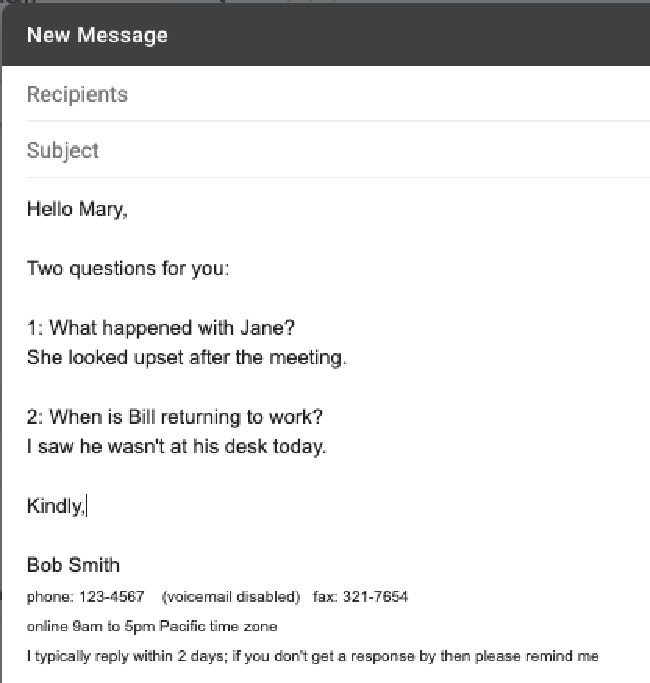
\includegraphics[width=1\textwidth]{images/email_two_questions.pdf}
\caption{Distinct items the recipient should address in a reply. A good subject for this email would indicate there are two questions you are seeking answers for.}
\label{fig:email_two_questions}
\end{figure}

\ \\
\textit{Email Tip}: If an item corresponds to a requested action, separately highlight the action and indicate who is supposed to take the action and what the deadline for response is.

\begin{figure}
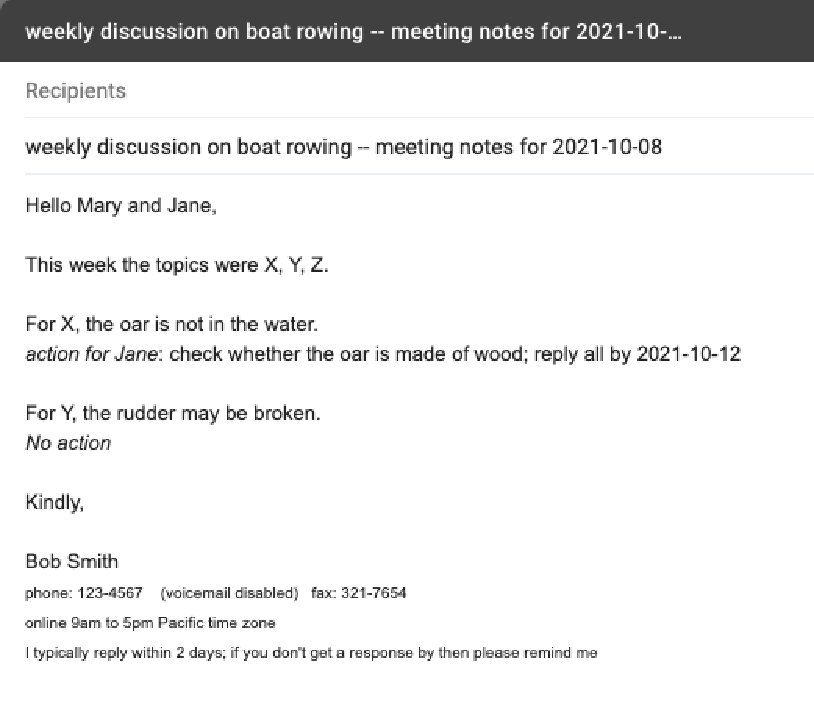
\includegraphics[width=1\textwidth]{images/email_meeting_notes.pdf}
\caption{Who has what action due when? The meeting notes are for a particular instance of a recurring event, so YYYY-MM-DD is included in the subject.}
\label{fig:email_meeting_notes}
\end{figure}

\ \\
\textit{Email Tip}: Computer commands should be distinct separate fixed-width font. This distinguishes the text from the rest of the narrative. 


\begin{figure}
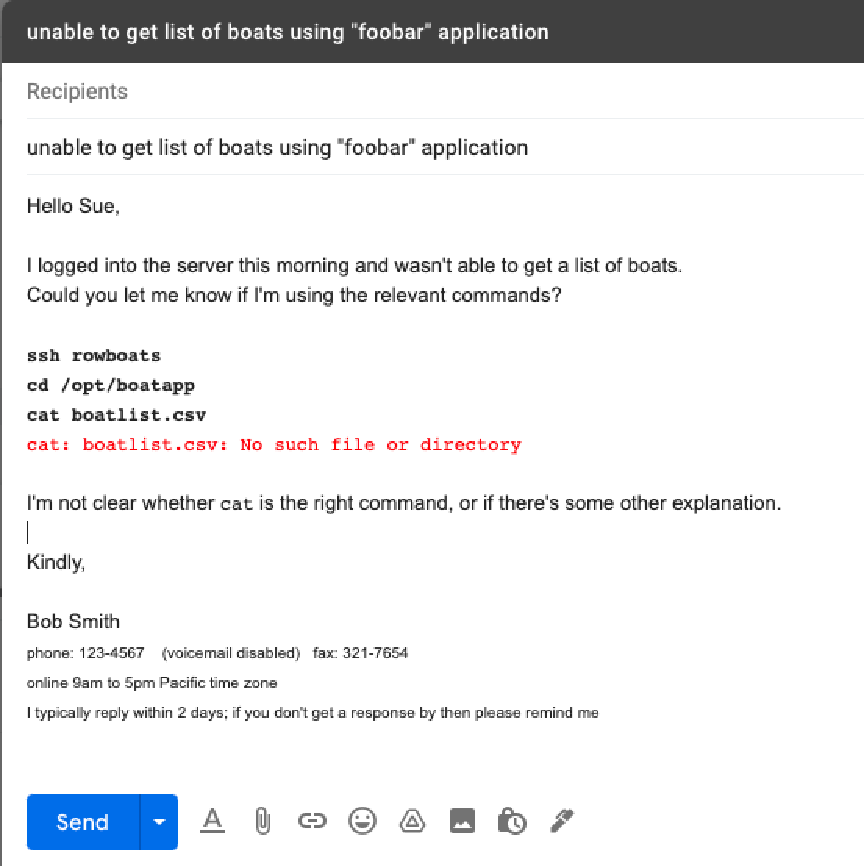
\includegraphics[width=1\textwidth]{images/email_computer_font.pdf}
\caption{The computer commands use fixed width font. The author distinguished input from output through the use of bold vs non-bold respectively. The author highlighted the error message using red. Inline text like ``cat'' in the last line is also fixed width.}
\label{fig:email_computer_font}
\end{figure}

\ \\
\textit{Email Tip}: References to documents include a direct full path.

\ \\
\textit{Email Tip}: If referring to a previous separate thread, include the subject and the date+time that email was sent

\ \\
\textit{Email Tip}: For bullet points, explicitly specify that items are joined by one of the following: OR, XOR, AND.

\ \\
\textit{Email Tip}: If you have an unordered list, explicitly state that order is irrelevant.

\ \\
\textit{Email Tip}: If you have a sequence of steps, number them and indicate which steps are required versus optional

\ \\
\textit{Email Tip}: Use visual sketches to illustrate concepts rather than always relying on text. Don't use pictures all the time, and don't have too many pictures in an email. 

\ \\
\textit{Email Tip}: Know how to both embed pictures inline and how to attach files and when to use which. 
Email replies should preferentially be at the top of the thread. 
If replying to multiple points in the previous email, embed replies inline, mark the distinction, and highlight the authorship. 

\begin{figure}
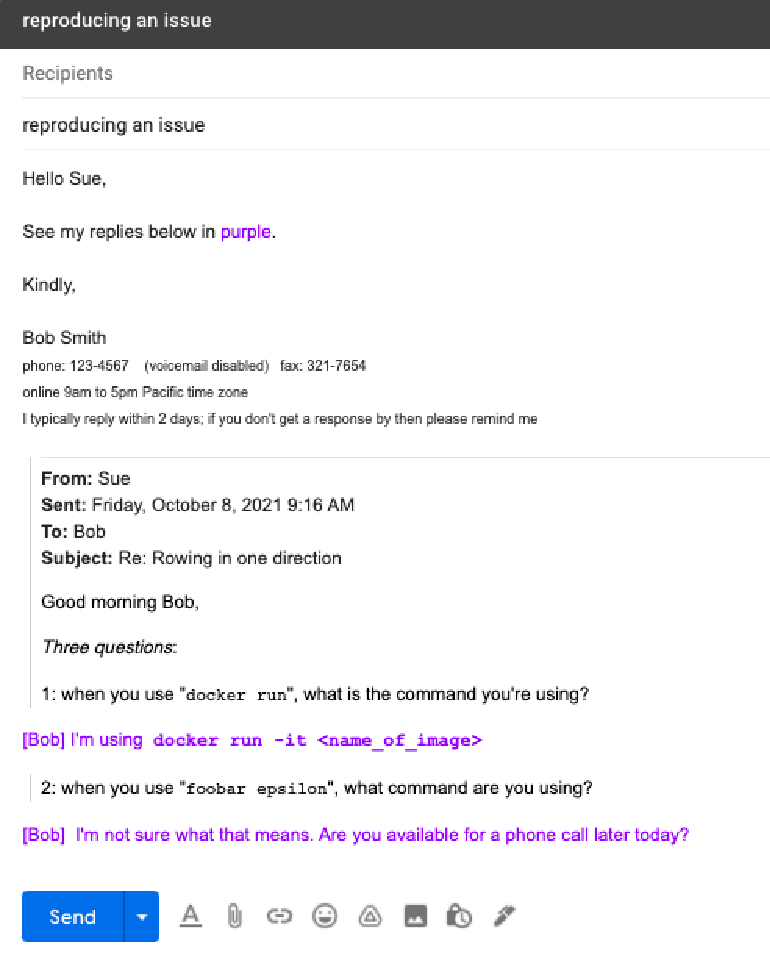
\includegraphics[width=1\textwidth]{images/email_reply.pdf}
\caption{Bob's reply to Sue's questions. The third question is not shown in this illustration.}
\label{fig:email_reply}
\end{figure}

\ \\
\textit{Email Tip}: If replying inline, explicitly state that at the top of the thread.

\ \\
\textit{Email Tip}: If the email is longer than a paragraph, provide a \href{https://en.wikipedia.org/wiki/BLUF_(communication)}{B.L.U.F} 
\index{\href{https://en.wikipedia.org/wiki/BLUF_(communication)}{BLUF}}
or 
\href{https://en.wikipedia.org/wiki/Wikipedia:Too_long;_didn\%27t_read}{tl;dr} 
\index{Wikipedia!\href{https://en.wikipedia.org/wiki/Wikipedia:Too_long;_didn\%27t_read}{tl;dr}}
or summary. In general emails should be short. Longer discussions should be held on the phone or in person, with a summary report after the discussion. Reliance on a BLUF or tl;dr risks resulting in the reader skipping the content. 

\ \\
\textit{Email Tip}: Every email should have a purpose. What are you asking the recipient to do? How do you want them to feel? How should they respond?

\ \\
\textit{Email Tip}: When replying, starting your email with an expression of gratitude for the work the recipient has done so far sets a positive tone by acknowledging their investment.

\ \\
\textit{Email Tip}: Read each email and report to determine the purpose. If you don't have time to read everything, skim the content. 
% https://graphthinking.blogspot.com/2021/03/read-each-email-to-determine-purpose.html

\textit{Problematic behavior}: First you scan the text of a message to see if there is immediate action or response needed. If no action or response is needed, go to the next email. \\
That may not work for emails that have logistics associated with future events, or emails that alter your perception of the situation.


If you read an email to figure out the purpose of the email, that will help determine what action and response are relevant. Here I'm using ``action" to refer to activities outside the email channel. 


\subsection*{Why did this Email get sent?}
Below are potential intentions of the person writing the email. 

\ \\
\textit{Email intent}: \textbf{Decision needed}. Typically includes context. \\
\textit{Action}: if the team maintains a decision log, update that.
Response is selection of a choice.

\textit{Tip}: Instead of asking for a decision, ask if the person is opposed. See 
\hyperref[sec:approval-forgiveness-opposition]{approval and forgiveness and opposition}
\marginpar{See page~\pageref{sec:approval-forgiveness-opposition}.}
for more details.

\textit{Tip}: Instead of asking for a decision, ask for the go-ahead. This framing biases the respondent towards action (specifically approval) rather than thinking. 

\ \\
\textit{Email intent}: \textbf{Situational awareness}.\\
\textit{Action}: Expected default is no action, but interject if there's an issue.

\ \\
\textit{Email intent}: \textbf{Action or Tasking}.\\
\textit{Action}: Do something within a specified deadline.

\ \\
\textit{Email intent}: \textbf{Approval sought}.\\
\textit{Action}: Confirm or deny.

\ \\
\textit{Email intent}: \textbf{Feedback sought}.\\
\textit{Action}: Assessment of proposal.

\ \\
\textit{Email intent}: \textbf{Meeting logistics}. Can be an announcement (widely available), registration (limited attendance), or invitation (specific to you). Attendance is either optional or required. \\
\textit{Action}: Create or update a calendar event.
Response should restate the logistics (specifically the time and date and location and purpose) to confirm. 

\ \\
\textit{Email intent}: \textbf{Brainstorming}\\
May provoke a response for building on an idea.
``For your situational awareness, no action needed." Notification of activity by someone else. Or change in plans. 
If needed, a correction to the described direction might trigger a response or even a meeting.

\ \\
\textit{Email intent}: \textbf{Reference} e.g. describing a process, or a business workflow, or a citation.\\
\textit{Action}: Copy process documentation to wiki. Copy citation to bibliography.
Acknowledgement response thanking the sender for the update or clarification.

\ \\
\textit{Email intent}: \textbf{Setting a formal policy or issuing an informal edict}.\\
\textit{Action}: move the policy or edict documentation to \href{https://en.wikipedia.org/wiki/Confluence_(software)}{Confluence}
\index{Wikipedia!\href{https://en.wikipedia.org/wiki/Confluence_(software)}{Confluence}}
or Wiki.
Acknowledgement response needed only if the edit is aimed at just me or the group I am leading.

\ \\
\textit{Email intent}: \textbf{Question}.\\
If this is a recurring question, move to a ``Frequently Asked Questions" page on a Confluence or Wiki.
Response needed that provides answer or seeks clarification.




